\documentclass[11pt, oneside]{article}
\usepackage[a4paper,bindingoffset=0.2in,%
            left=1in,right=1in,top=1in,bottom=1in,%
            footskip=.25in]{geometry}
\usepackage{graphicx}
\usepackage{enumerate}
\usepackage{url}
\usepackage{hyperref}
\usepackage{pbox}
\usepackage{CJKutf8}
\usepackage{mathtools}
\usepackage{microtype}
\usepackage[htt]{hyphenat}
\renewcommand{\vec}[1]{\mathbf{#1}}


\begin{document}
\title{Assignment 1: Regression and KNN (part III)}
\author{Xiyou Zhou, 13307130189 \\ Computer Science and Technology}
\maketitle

\section{Logistic Regression}
First we use all 1 for weight initialization. We used four kinds of preprocessing methods and different $\lambda$ values for models. The results are shown as plots below or in the appendix.

The error rate at different $\lambda$ values is as follows.

\begin{table}[h]
\centering
\caption{Training Error}
\begin{tabular}{l|lll}
\hline
preprossing & $\lambda$ = 1     & $\lambda$ = 10    & $\lambda$ = 100   \\
\hline
none       & 43.49 & 58.47 & 38.86 \\
znormalize & 10.47 & 10.38 & 9.27  \\
binarized  & 12.10 & 11.91 & 10.70 \\
log        & 6.82  & 6.88  & 54.75 \\
\hline
\end{tabular}
\end{table}

\begin{table}[h]
\centering
\caption{Test Error}
\begin{tabular}{l|lll}
\hline
preprossing & $\lambda$ = 1     & $\lambda$ = 10    & $\lambda$ = 100   \\
\hline
none       & 45.31 & 59.38 & 37.17 \\
znormalize & 11.07 & 10.94 & 9.70  \\
binarized  & 11.13 & 11.26 & 10.81 \\
log        & 7.75  & 8.14  & 56.25 \\
\hline
\end{tabular}
\end{table}

Generally speaking, as $\lambda$ increases, training error and test error drops like in z-normalize and binarized method. This is probably because the parameters are restricted to better fit the data instead of wasting gradient descents on local minimal. log preprocessing seems to reach the best performance with 6.82\% training error and 7.75\% test error, but the penalize of $\lambda$ makes the model underfit and reaches very bad accuracy. With no preprocessing, the model performance is very random and bad. I think it is because the very non-uniform distribution of feature scale and not tuned initial weight.

With preprocessing method changes, the performance varies a lot. No preprocessing gives very bad accuracy and random result. Z-normalize reaches less than 10\% error rate and training error is always less than test error. Binarized processing also reaches error rate close to 10\% but the test error is more steady than training error and their relationship changed during the change of $\lambda$. Log preprocessing method gives very unsteady results. It can reach very great accuracy at some $\lambda$ while it underfits when $\lambda$ is too large. The test accuracy is always close to training accuracy, thus more training epochs would definitely make the results more steady.

After all, log preprocessing method provided best result and converged the most quickly.


\section{Linear Regression}

Using linear least squares to compute weight for linear regression, we can see the results from plots with different preprocessing methods below or in the appendix.

The error rate at different $\lambda$ values is as follows.

\begin{table}[h]
\centering
\caption{Training Error}
\begin{tabular}{l|lll}
\hline
preprossing & $\lambda$ = 1     & $\lambda$ = 10    & $\lambda$ = 100   \\
\hline
none       & 10.57 & 10.15 & 10.15 \\
znormalize & 10.57 & 10.41 & 9.56  \\
binarized  & 7.31 & 7.31 & 7.31 \\
log        & 6.10  & 6.04  & 6.04 \\
\hline
\end{tabular}
\end{table}

\begin{table}[h]
\centering
\caption{Test Error}
\begin{tabular}{l|lll}
\hline
preprossing & $\lambda$ = 1     & $\lambda$ = 10    & $\lambda$ = 100   \\
\hline
none       & 12.11 & 11.59 & 11.52 \\
znormalize & 12.04 & 11.59 & 11.39  \\
binarized  & 7.81 & 7.81 & 7.81 \\
log        & 6.51  & 6.58  & 6.45 \\
\hline
\end{tabular}
\end{table}

As $\lambda$ increases, training error and test error drops in all preprocessing methods. In not preprocessed method, training error does not change but test error drops as result of regularization. Binarized preprocessing method provided unchanging results.

Log preprocessing method gives the best results, even better than Logistic Regression method. Binarized results is steady, the training error and test error stayed around 7\%. Other methods have error rate around 10\% and clearly larger test error than training error.

Tried the SGD plot, but result not ideal, will ask the TA later.

\section{K-Nearest Neighbors}

The plots of training and test error as K changes can be seen below or in the appendix.
Here's the error rate at K = 1, 10, 100.
\begin{table}[h]
\centering
\caption{Training Error}
\begin{tabular}{l|lll}
\hline
preprossing & K = 1     & K = 10    & K = 100   \\
\hline
none       & 0.03 & 18.24 & 25.61 \\
znormalize & 0.03 & 8.25 & 12.46  \\
binarized  & 4.47 & 10.15 & 11.39 \\
log        & 0.03  & 5.29  & 8.91 \\
\hline
\end{tabular}
\end{table}

\begin{table}[h]
\centering
\caption{Test Error}
\begin{tabular}{l|lll}
\hline
preprossing & K = 1     & K = 10    & K = 100   \\
\hline
none       & 17.97 & 22.07 & 24.67 \\
znormalize & 9.64 & 10.09 & 13.93  \\
binarized  & 14.84 & 12.04 & 12.5 \\
log        & 6.51  & 7.03  & 10.55 \\
\hline
\end{tabular}
\end{table}

As K increases, error rate generally also increases except binarized data. When K = 0, binarized preprocessing method gives a very high training error rate because there are too many data with same different bits. Other preprocessing method gives a training error rate almost equal to 0 but not 0. I think that's because some small contradiction inside dataset or float error.

With none preprocessing, log or znormalize, all training and test error rate increases as K increases. Z and log preprocessing always have larger training error and none preprocessing have test error even larger than training error at large K. In binarized preprocessing method, the error rate converges at large K, training and test error tend to be closer as K increases.

\newpage
\section{Survey}
12 hours in 3 days.

\begin{thebibliography}{9}
\bibitem{CourseraLR}
Coursera, Machine Learning, Lecture 43 - Regularized Logistic Regression
\\\texttt{https://www.coursera.org/learn/machine-learning/lecture/4BHEy/regularized-logistic-regression}

\bibitem{cmulrbook}
CMU Statistics, Undergraduate Advanced Data Analysis, Logistic Regression
\\\texttt{http://www.stat.cmu.edu/\~{}cshalizi/uADA/12/lectures/ch12.pdf}

\bibitem{uwlecppt}
University of Washington, L2 Regularization for Logistic Regression
\\\texttt{http://courses.cs.washington.edu/courses/cse599c1/13wi/slides/l2-regularization-online-perceptron.pdf}

\bibitem{stfufldl}
Stanford, UFLDL Tutorial, Logistic Regression
\\\texttt{http://ufldl.stanford.edu/tutorial/supervised/LogisticRegression/}

\bibitem{mlapp}
Machine Learning, A Probabilistic Perspective, p16-17:\\A simple non-parametric classifier: K-nearest neighbors
\\\texttt{https://www.cs.ubc.ca/\~{}murphyk/MLbook/pml-intro-22may12.pdf}
\end{thebibliography}

\newpage
\section{Appendix}

\begin{figure}[h]
\centering
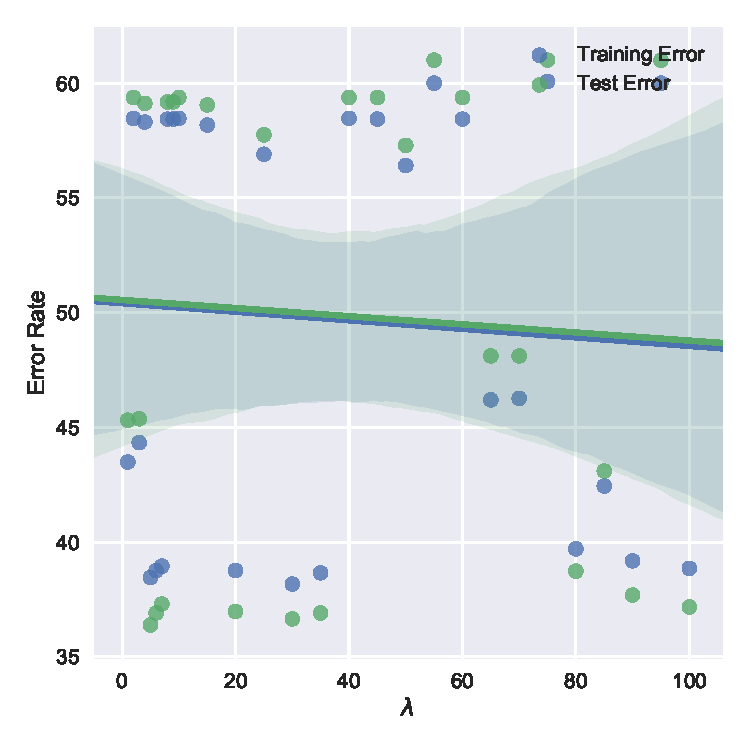
\includegraphics{foo_.pdf}
\caption{Plot of Logistic Regression Training \& Test error after 100 epochs with no preprocessing}
\end{figure}

\begin{figure}[h]
\centering
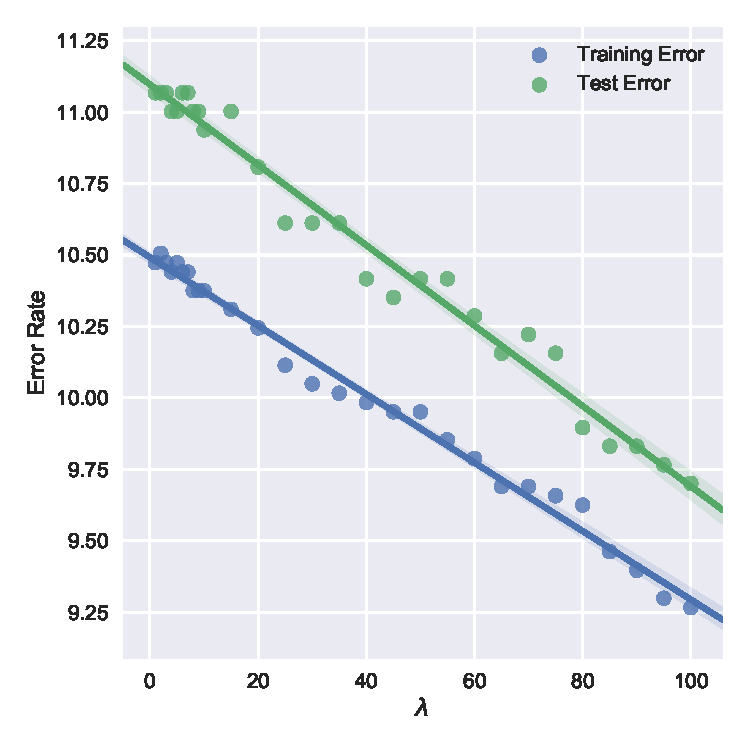
\includegraphics{foo_z.pdf}
\caption{Plot of Logistic Regression Training \& Test error after 100 epochs with z-normalize preprocessing}
\end{figure}

\begin{figure}[h]
\centering
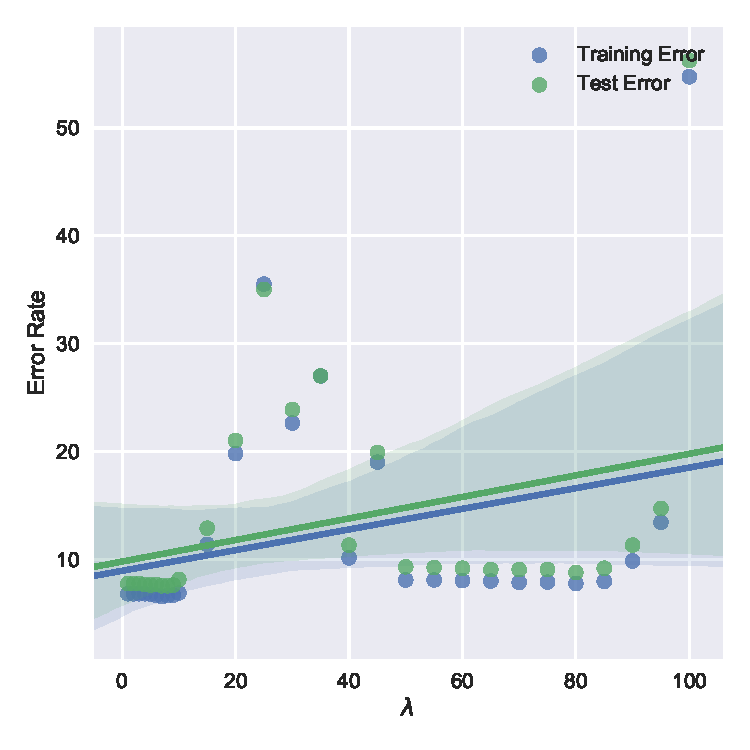
\includegraphics{foo_log.pdf}
\caption{Plot of Logistic Regression Training \& Test error after 100 epochs with log preprocessing}
\end{figure}

\begin{figure}
\centering
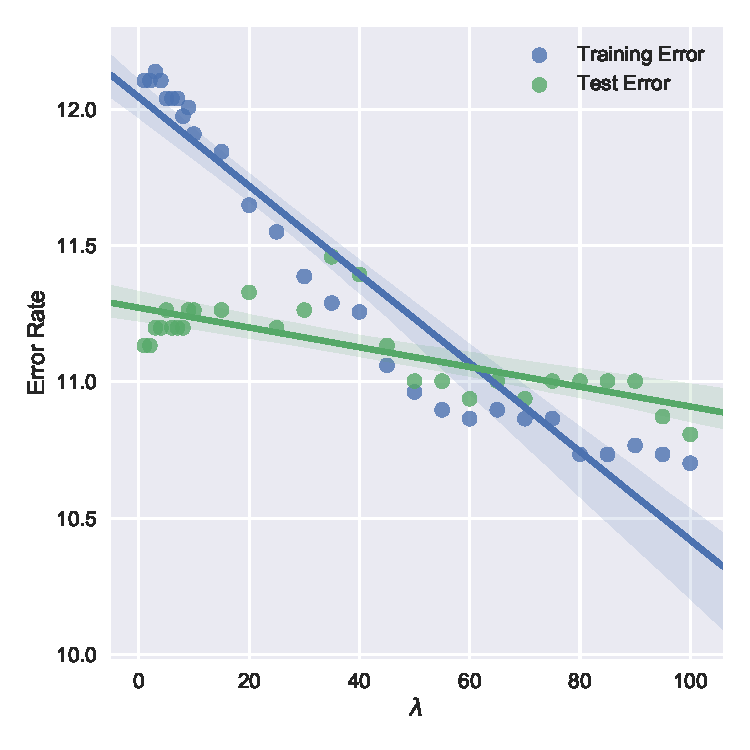
\includegraphics{foo_binarized.pdf}
\caption{Plot of Logistic Regression Training \& Test error after 100 epochs with binarized preprocessing}
\end{figure}

\begin{figure}[h]
\centering
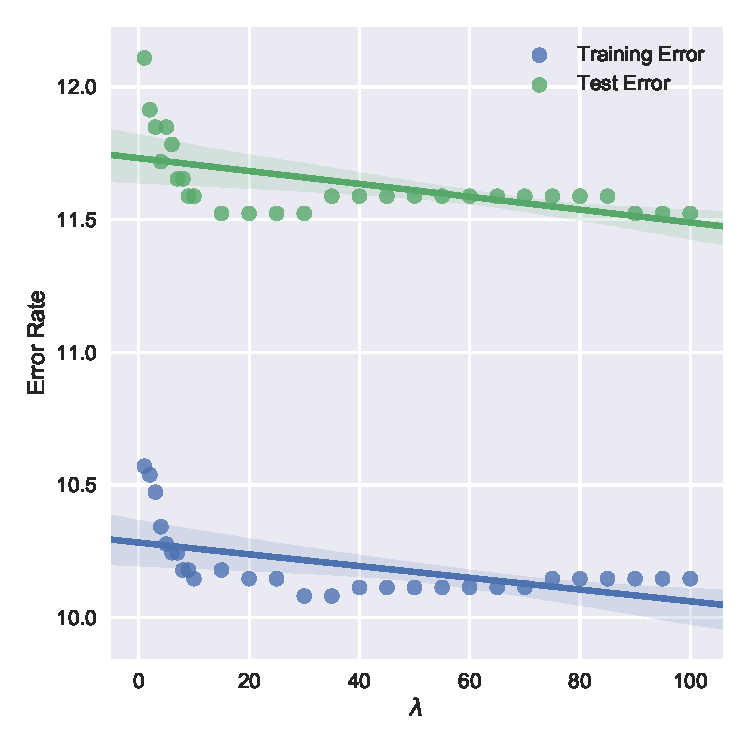
\includegraphics{linear_.pdf}
\caption{Plot of Linear Regression Training \& Test error with linear least squares and no preprocessing}
\end{figure}

\begin{figure}[h]
\centering
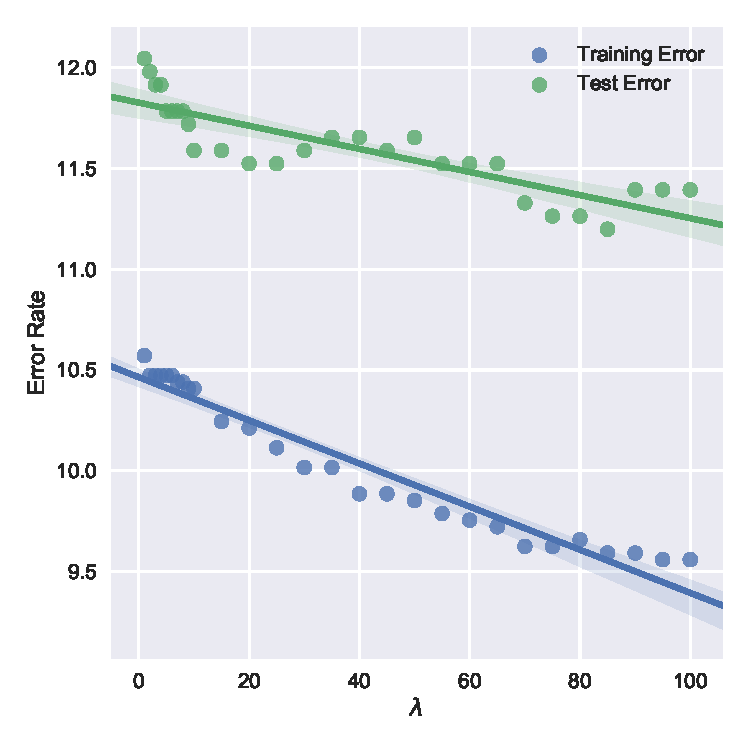
\includegraphics{linear_z.pdf}
\caption{Plot of Linear Regression Training \& Test error with linear least squares and z-normalize preprocessing}
\end{figure}

\begin{figure}[h]
\centering
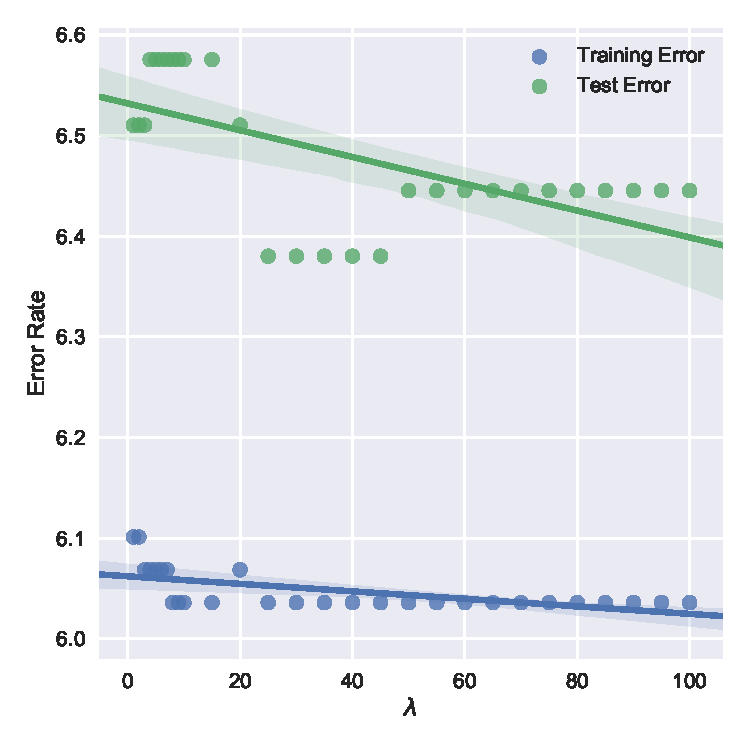
\includegraphics{linear_log.pdf}
\caption{Plot of Linear Regression Training \& Test error with linear least squares and log preprocessing}
\end{figure}

\begin{figure}[h]
\centering
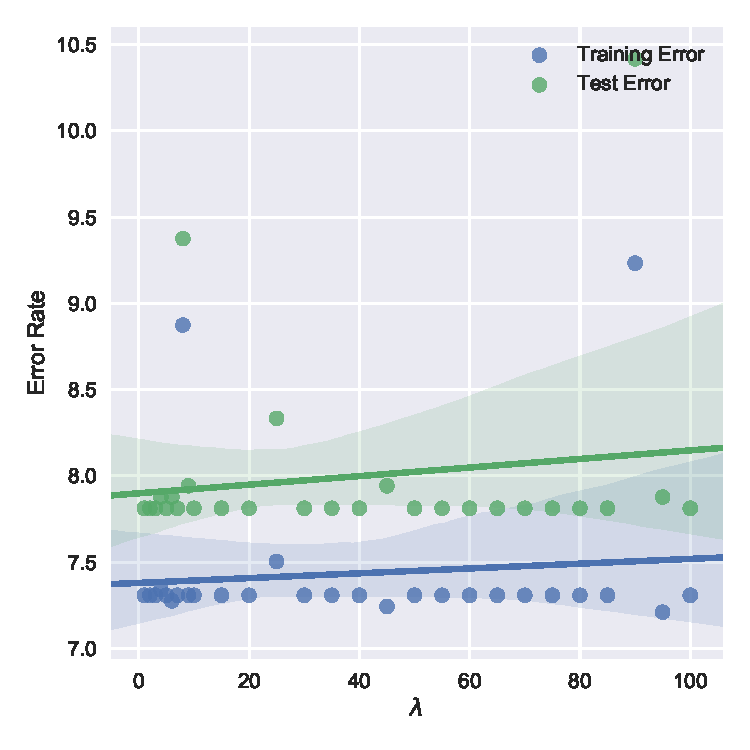
\includegraphics{linear_binarized.pdf}
\caption{Plot of Linear Regression Training \& Test error with linear least squares and binarized preprocessing}
\end{figure}

\begin{figure}[h]
\centering
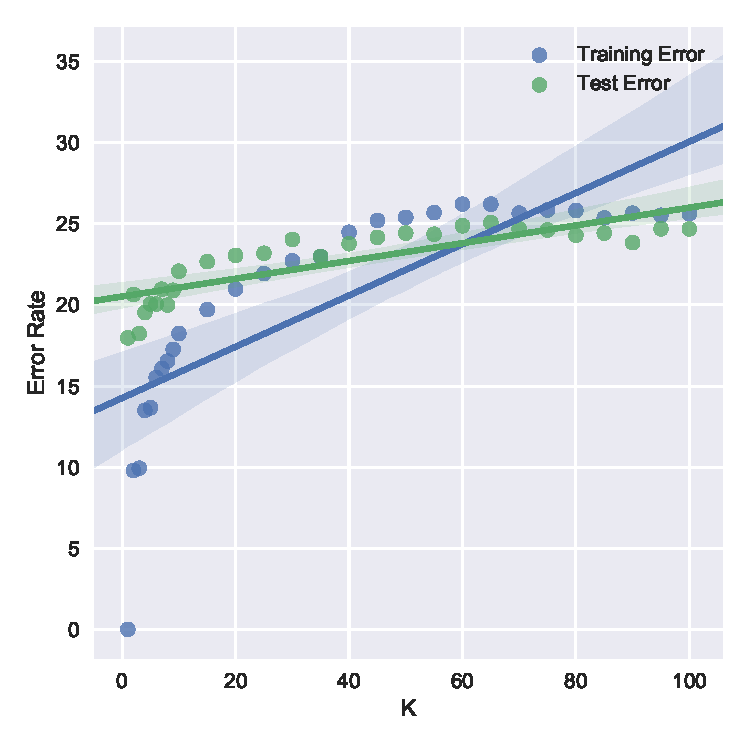
\includegraphics{knn_.pdf}
\caption{Plot of K-Nearest Neighbor Classifier Training \& Test error with no preprocessing}
\end{figure}

\begin{figure}[h]
\centering
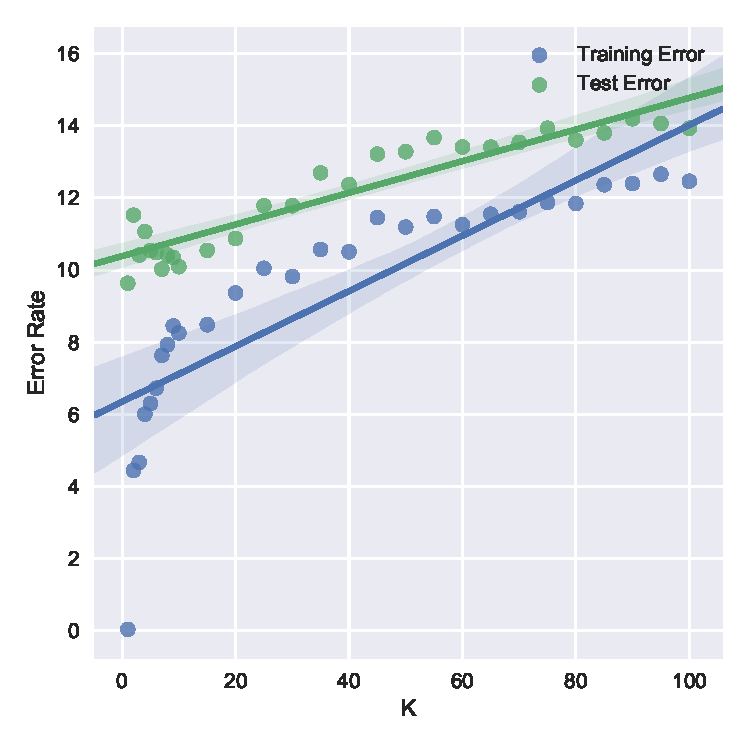
\includegraphics{knn_z.pdf}
\caption{Plot of K-Nearest Neighbor Classifier Training \& Test error with z-normalize preprocessing}
\end{figure}

\begin{figure}[h]
\centering
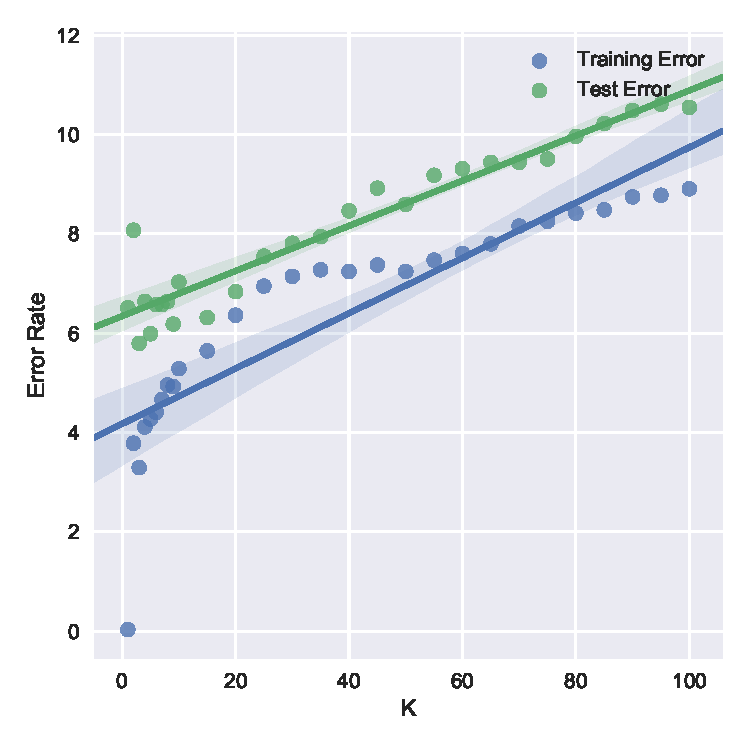
\includegraphics{knn_log.pdf}
\caption{Plot of K-Nearest Neighbor Classifier Training \& Test error with log preprocessing}
\end{figure}

\begin{figure}[h]
\centering
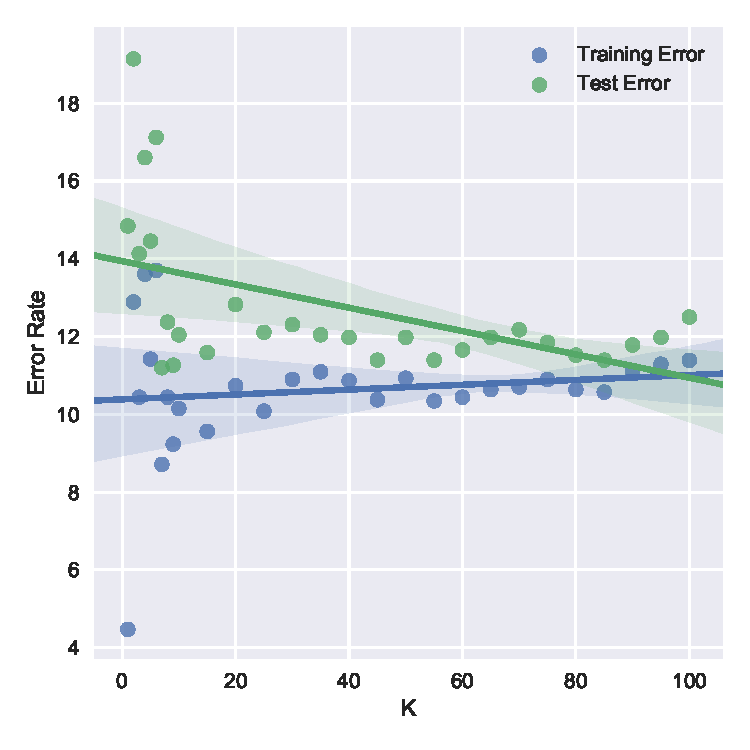
\includegraphics{knn_binarized.pdf}
\caption{Plot of K-Nearest Neighbor Classifier Training \& Test error with binarized preprocessing}
\end{figure}

\end{document}